\section{Introduction}

\subsection{Du résumé à la reconstruction}

Lire un article, c’est repérer ce qu’il affirme, ce qui justifie chaque affirmation et les objections auxquelles il répond. Les assistants fondés sur des modèles de langage (LLM) proposent surtout des résumés. Un résumé condense le contenu, mais il ne rend pas inspectables les dépendances entre propositions. Il n’est pas non plus toujours fidèle : sur 4\,900 résumés produits par dix modèles, \textcite{ref30} observent des généralisations plus larges que celles des textes d’origine, dans 26 à 73~\% des cas pour trois des modèles étudiés, et près de cinq fois plus souvent que dans des résumés écrits par des humains. Un lecteur qui veut juger un raisonnement a besoin d’en voir la structure et de pouvoir remonter, pour chaque pas, à la phrase qui le fonde.

Le sujet du projet demande un outil de ce type : extraire d’un texte les concepts, les arguments, les exemples, les positions adverses et les conclusions ; repérer des motifs de raisonnement (divergence, convergence, contradiction, raffinement, causalité) ; les montrer sous forme de carte ou de \emph{storyline} qui suive l’évolution des idées dans le texte ; retrouver d’un clic le passage d’origine de chaque élément ; tester l’ensemble sur des textes philosophiques, scientifiques et des essais. Visual Reasoning Maps est le prototype réalisé pour y répondre. Il présente un aperçu de cinq à douze étapes, développables en sous-étapes, et affiche pour chaque étape les phrases citées dans la mise en page d’origine du document (figure~\ref{fig:prototype}).

\begin{figure}[t]
\centering
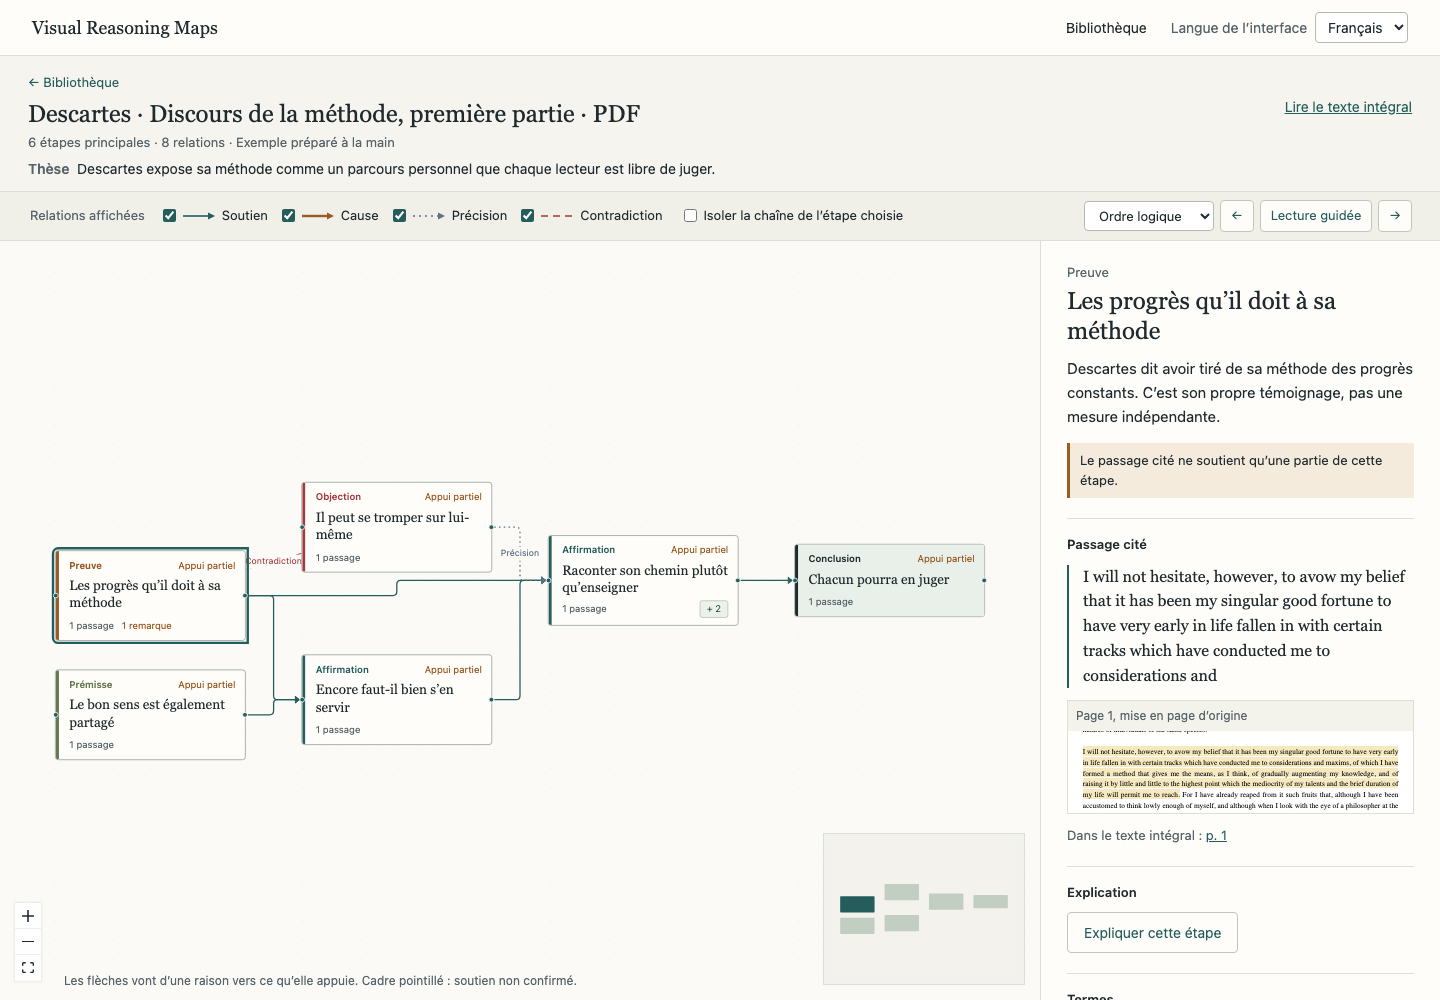
\includegraphics[width=\textwidth]{figures/carte-descartes.png}
\caption{Le prototype sur l’exemple fourni avec le dépôt, la première partie du \emph{Discours de la méthode} dans une traduction anglaise du domaine public. À gauche, la carte des étapes principales ; à droite, l’étape sélectionnée, son statut et le passage cité dans sa mise en page d’origine. Cet exemple a été préparé à la main.}
\label{fig:prototype}
\end{figure}

\subsection{Questions}

Quatre questions organisent la revue :
\begin{enumerate}
  \item Quelles unités et quelles relations extraire, et avec quelle fiabilité un modèle peut-il le faire ?
  \item Comment les disposer pour donner une vue d’ensemble sans couper le lecteur du texte ?
  \item Comment rattacher chaque élément au texte, et comment contrôler ce rattachement ?
  \item Comment évaluer un tel système, sachant que le modèle qui produit la carte ne peut pas en être le seul juge ?
\end{enumerate}

\subsection{Corpus et méthode}

Le point de départ est une liste de 23 références fixée au lancement du projet, accompagnée d’une lecture facultative, la revue de \textcite{ref12b} sur le regroupement d’arêtes, que nous avons retenue. Nous y avons ajouté huit sources pour combler des manques apparus pendant la rédaction : la théorie de l’argumentation et du discours \parencite{ref24,ref25,ref26}, un principe classique de conception d’interfaces de visualisation \parencite{ref27}, la vérification d’affirmations scientifiques \parencite{ref28}, la fiabilité des LLM employés comme juges \parencite{ref29}, la fidélité des résumés scientifiques produits par des LLM \parencite{ref30} et la documentation de l’algorithme de disposition utilisé par le prototype \parencite{ref31}. La revue n’est donc pas systématique.

Les textes ont été lus en intégralité quand ils étaient librement accessibles. Quatre ne l’ont été qu’à travers leur résumé et leurs métadonnées \parencite{ref09,ref10,ref12,ref12b} : nous ne leur prêtons rien de plus. Les références renvoient aux versions publiées ; lorsque la version lue est une prépublication, les pages citées sont celles de cette version. Chaque source a une fiche de lecture (dossier \texttt{paper/fiches} du dépôt) qui indique la version consultée, les pages utilisées et ce qui reste à vérifier. Les sources ont été consultées les 22 et 23 septembre 2026.

\subsection{Plan}

La section~\ref{sec:notions} précise ce que la carte représente. Les sections~\ref{sec:extraction} à~\ref{sec:critique} traitent successivement de l’extraction de la structure, de sa représentation, de son ancrage dans le texte et de la critique automatique. La section~\ref{sec:synthese} compare les systèmes étudiés, en tire six exigences et situe le prototype ; la section~\ref{sec:evaluation} décrit le protocole d’évaluation prévu.
